\chapter{Approach: The non-equilibrium Green's Function formalism}
\label{ch:chapter_2}

\begin{abstract}
In this chapter, I derive the non-equilibrium Green's Function Formalism, the Dyson and Keldysh Equations, and several other useful quantities. I will look explicitly at properties of interest, such as the occupation of the levels of and the current through the molecule.
\end{abstract}

%% Start the actual chapter on a new page.
\newpage
\section{Introduction}
Any closed quantum mechanical system can in principle be described by the Schr\"o\-dinger equation. For such a system, there are several methods for solving the many-body Schr\"o\-dinger equation, for instance the popular Hartree-Fock (HF) and density-functional theory (DFT) quantum chemistry methods.

However, our systems of interest are not closed. A molecule is coupled to metallic electrodes, which connect to a voltage source. The circuit is further extended with measurement equipment, refrigeration instruments and so forth. The system might also not be in equilibrium, such as when a bias voltage is applied between the two electrodes. Such a system cannot be described by a Hamiltonian \cite{seldenthuis}.

Green's functions are a familiar concept in partial differential equations. Green's functions characterise a partial differential equation completely, allowing you to obtain a solution for any given initial and boundary conditions and possible forcing terms rather easily, by integration. For instance, the Green's function for the Heat Equation $G(x,t; x_0, t_0)$ expresses the influence of the heat supplied at $(t_0, x_0)$ on the temperature at $(t,x)$ \cite{haberman}. 
While I will try to give a self-contained derivation of the non-equilibrium Green's Function formalism, I refer the reader to Refs.~\cite{mattuck,diventra,haugjauho, leeuwen} for a more complete overview.

For a closed system in equilibrium, the Green's Function formalism is exact because it is simply a rephrasing of the Schr\"odinger equation. However, the non-equilibrium Green's Function formalism also provides a systematic approach to incorporate some non-equilibrium interactions of nanoscopic systems with infinitely large environments, which is still exact in some limit. It is perhaps illuminating to first go over a number of assumptions and approximations \cite{seldenthuis}. 

First, the metallic electrodes or leads are considered as infinite reservoirs that are non\hyp{}interacting and are in equilibrium and not influenced by the molecule. Note that the leads are not required to be in equilibrium with each other. Although the immediate environment of the molecule is likely to be influenced by the molecule, it is possible to partition the system. The Extended Molecule which includes the lead-tips in addition to the molecule, allows for including  molecule-lead influences. Second, there is an assumption of adiabatic temporal evolution, so that the system in the infinite past can be considered as two isolated leads and molecule.  Finally, the system is an open quantum system. Electrons travel to the leads and move into an infinite reservoir, thus losing all information of their dynamics. 

These three approximations or assumptions are sufficient to obtain closed expressions for the properties of interest. However, as usual the equations become unwieldy for systems that approach the complexity of an actual laboratory nanoscopic system, requiring unrealistic computational resources.

It is for this reason that other approximations are employed for practical applications, such as the mean-field approximation. In this approximation, the interactions are essentially averaged out, which makes \emph{ab initio} quantum transport problems feasible. However, you lose certain transport phenomena, most notably the \emph{Coulomb Blockade} (section~\ref{sec:capacitive}).

This chapter is set up as follows. First, I will consider the many-body Schr\"odinger equation in section~\ref{sec:schrodinger}. I will then introduce Slater determinants and move on to the Fock-space and the formalism of second quantisation in section~\ref{sec:secondquantisation}. I will then derive the application of the Green's Functions in section~\ref{sec:greensfunctions}. How to find the form of the Green's Functions will be discussed in section~\ref{sec:eommethod}. Separately, I discuss how that method can be applied to find the tunnelling contribution to the Green's Functions in section~\ref{sec:tunnelling}.

Finally, I discuss how to find properties of interest in section~\ref{sec:properties} and the common application of the formalism in section~\ref{sec:synthesis}.

\section{Many Body Schr\"odinger Equation}
\label{sec:schrodinger}

For an arbitrary number $N$ of particles, both electrons and others, the many-body Schr\"o\-dinger equation is:
\begin{align}
 \imath \hbar \partial_t\ket{\Psi\left(t, r_0^\mu, r_1^\mu, \ldots r_N^\mu\right)} &= \widehat{H} \ket{\Psi\left(t, r_0^\mu, r_1^\mu, \ldots r_N^\mu\right)} \label{eq:schrodinger}, \\
 H &\equiv V\left(t, r_0^\mu, r_1^\mu, \ldots r_N^\mu\right) - \sum_{i=0}^N \frac{\hbar^2}{2m_i} \nabla_i^2.
\end{align}

It is clear that for many-particles ($N\gg 1$), equation~\ref{eq:schrodinger} becomes too complex rather rapidly. We will need some approximations before it becomes applicable.

If we consider the Hilbert space of atoms $H_A$ and that of electrons $H_e$, then their composite Hilbert space is $H = H_A \otimes H_e$. If the basis of $H_A$ is $\ket{\phi_i}$ and that of $H_e$ is $\ket{\psi_j}$, then an arbitrary state is:
\begin{align}
\ket{\Psi} &= \sum_{ij} c_{ij} \ket{\phi_i} \otimes \ket{\phi_j}.
\end{align}

Such a state is separable if  $\ket{\Psi}$ can be written as $\ket{\Psi_A} \ket{\Psi_e}$, where $\ket{\Psi_A}$ is a vector in the atomic space and $\ket{\Psi_e}$ is a vector in the electron space. An alternative formulation is that states that are separable are not entangled.

The Born-Oppenheimer approximation is based on the assumption that the electron and atom  states are separable \cite{mattuck}. It is justified because atoms are about three orders of magnitude more massive than electrons, and thus they are expected to move much more slowly. The convenience of the Born-Oppenheimer approximation is that the effect of the atoms, i.e. that of the molecular skeleton, is to provide an effective background potential for the electronic wave functions.

The Hamiltonian then reduces to the following effective electron-only form:
\begin{align}
H_e &= \sum_i \frac{p_i^2}{2m} + V_A + H',
\end{align}
where $V_A$ is the effective atomic background potential and $H'$ simply describes the interactions.

\section{Second Quantisation}
\label{sec:secondquantisation}
Consider a single-particle (fermion) Hilbert space $H_{sp}$, with the wave function or states of the $i$-th particle at momentum $k_j$ denoted $\ket{\phi_{k_j}(r_i)}$\footnote{I do not literally write down the spin of a state. Consider it the convention that spin is included in the labelling of the states, i.e. $k \rightarrow \sigma, k$.}. The full electron Hilbert space $H_e$ is defined by successive tensor products $H_{e} = H_{sp} \otimes H_{sp} \otimes \ldots \otimes H_{sp}$, so that the separable single-particle wave function products still span the space $H_e$. However, the symmetry requirements of the Pauli exclusion principle have to be satisfied, leading to the Slater determinant for $N$ particles\cite{yuli}:
\begin{align}
\ket{\Phi_k} &= \frac{1}{\sqrt{{N-1}!}} \begin{vmatrix}
\ket{\phi_{k_0}(r_0^\mu)} & \ket{\phi_{k_0}(r_1^\mu)} &\ldots& \ket{\phi_{k_0}(r_{N-1}^\mu)} \\
\ket{\phi_{k_1}(r_0^\mu)} & \ket{\phi_{k_1}(r_1^\mu)} &\ldots& \ket{\phi_{k_1}(r_{N-1}^\mu)} \\
\ldots&\ldots&\ldots&\ldots&\\
\ket{\phi_{k_{N-1}}(r_0^\mu)} & \ket{\phi_{k_{N-1}}(r_1^\mu)} &\ldots& \ket{\phi_{k_{N-1}}(r_{N-1}^\mu)} \\
\end{vmatrix},
\label{eq:slaterdeterminant}
\end{align}
which describes a vector in the full Hilbert space $H_e$ with specific momentum. Note that the matrix must be $N\times N$. %If there are fewer states than particles, the Pauli exclusion principle cannot be satisfied. If there are more states than particles, then some are simply not occupied and shouldn't be in the product.

That leads us to the notion of a Fock state. A Fock state fully specifies a quantum many-body state by listing the occupied states. However, it does not tell you which particle is in what state, which fits the Slater determinant splendidly:
\begin{align}
\ket{\Phi_k} &= \ket{n_{k_0}, n_{k_1},\ldots, n_{k_M}},
\label{eq:fock}
\end{align}
where $M$ simply is the total number of single-particle states. The occupancy of each state is thus defined in the Fock state. A Fock space is just a direct sum of Hilbert spaces of any number of particles, i.e. $H = H_{N=0} + H_{N=1} + H_{N=2}\ + \ldots + H_{N=M}$. A basis of the Fock space is formed by all Slater determinants constructed from a single-particle basis. 

The Fock space is orthonormal:
\begin{align*}
\braket{ \left. \left\{ n_k \right\} \right| \left\{ n_k' \right\}} &= \prod_{k} \delta_{n_k}^{n_k'}.
\end{align*}

Similar to the ladder operator approach \cite{griffiths}, we can define the creation $d^\dagger_k$ and annihilation $d_k$ operators:
\begin{align*}
d_k^\dagger \ket{\ldots, 0_k, \ldots} &=\ket{\ldots, 1_k, \ldots},\\
d_k \ket{\ldots, 1_k, \ldots} &=\ket{\ldots, 0_k, \ldots}.
\end{align*}

Note that the commutator $\left\{ d_k, d_{k'}^\dagger\right\} = \delta_{kk'}$, while the commutators $\left\{ d_k, d_{k'}\right\}$ and $\left\{ d_k^\dagger, d_{k'}^\dagger\right\}$ are zero. The operator $n_k = d_k^\dagger d_k$ is called the number operator. 

The above technique is called second quantisation \cite{yuli}. Second quantisation allows for easy dealing with many-body Hamiltonians and Fock space, as any state can be created by a series of creation operators acting on a vacuum state $\ket{0}$. 
 

\section{Green's Functions}
\label{sec:greensfunctions}
In the following chapters, I largely follow \citet{seldenthuis} for a general treatment of the non-equilibrium Green's Function Formalism. As mentioned, for a complete derivation of the formalism, see Refs.~\cite{mattuck,diventra,haugjauho}.

We define the single-particle Green's function operator as:
\begin{align}
G_{ij} (t,t') &= -\frac{\imath}{\hbar} T\left\{d_i(t)d_j^\dagger(t')\right\},
\label{eq:greensfunction}
\end{align}
where $T$ is the time-ordering operator, which moves operators at earlier times to the right. In this definition, I specify the operator rather than the expectation value $\braket{G_{ij}(t,t')}$ which is used in practise. For a time-independent Hamiltonian, the Green's function will depend only on the time difference $t - t'$. 

The Green's function can be interpreted as a propagator. If a particle is created in state $\ket{i'}$ at time $t'$, the Green's function gives us the probability that it is found in state $\ket{i}$ at time $t$, i.e. that it propagated from $\ket{i'}$ to $\ket{i}$.

The main problem is finding a closed expression for the Green's function of a particular system. I will start out by approximating the full propagator $G_{ij}(t,t')$ with the free propagator $g_{ij}(t,t')$, the propagator in the absence of any interactions. 

\begin{figure}[!bt]
    \centering
    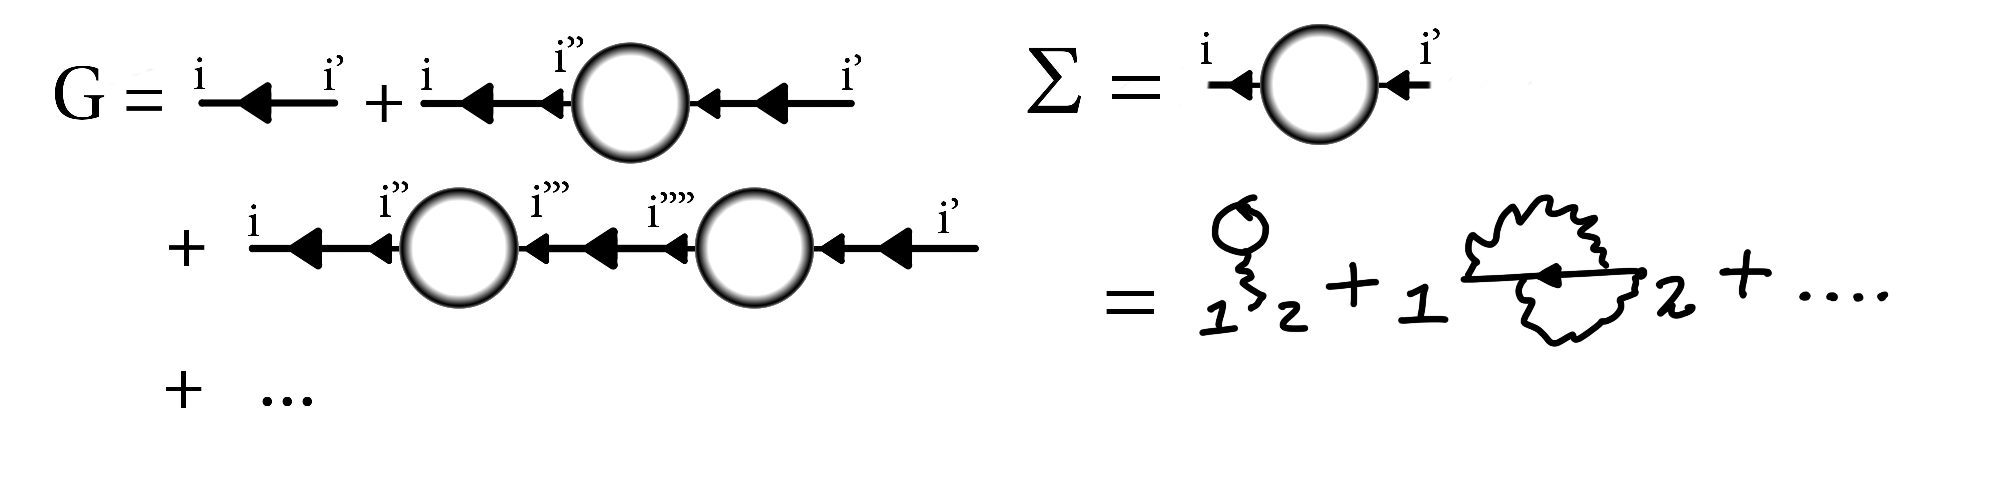
\includegraphics[width=\textwidth]{pdf/diagrams.pdf}
    \caption{Diagrammatic structure for the Green's function (left). The self energy (right) consists of all diagrams that do not break up into two disjoint pieces~\cite{leeuwen}.}
    \label{fig:firstorderdiagram}
\end{figure}
The full propagator does of course interact. But, it can be expanded diagrammatically \cite{mattuck}, as depicted in Figure~\ref{fig:firstorderdiagram}. By diagram, I am referring to Feynman diagrams, a technique in which mathematical expressions are expressed in a picture which should reduce abstractness. The first diagram is the free propagator (the arrow in Figure~\ref{fig:firstorderdiagram}). The second diagram is the first order approximation (arrow, self-energy, arrow in Figure~\ref{fig:firstorderdiagram}), where the particle moves from $\ket{i'}$ at time $t'$ to a different state $\ket{i''}$ at time $t''$, interacts with a potential and scatters to state $\ket{i'''}$ at time $t'''$ and finally propagates to $\ket{i}$ at time $t$. We could write this down in the time-domain, but it is far more convenient to write it down as a matrix equation in the energy (Fourier) domain:
\begin{align*}
G &= g + g \Sigma g,
\end{align*}
where $\Sigma$ is the self-energy, the sum of all possible interactions.

The second order term is of course when it propagates, scatters, propagates, scatters and propagates to the final state (arrow, self-energy, arrow, self-energy, arrow in Figure~\ref{fig:firstorderdiagram}):
\begin{align*}
G &= g + g \Sigma g + g \Sigma g \Sigma g.
\end{align*}

The continuation of these terms is very clear. It has a very nice solution, though:
\begin{align}
G &= g + g \Sigma g + g \Sigma g \Sigma g+ \ldots \nonumber\\
&= g + g \Sigma G. \label{eq:dyson}
\end{align}

This equation is known as the Dyson equation. We will see that the Dyson equation is of fundamental importance to transport calculations in section~\ref{sec:eommethod}.

Despite the possibility to analyse the system in terms of the single-particle Green's function, it is in practise preferred to define auxiliary Green's functions and use these to solve the problem:
\begin{itemize}
\item The lesser Green's function, 
\begin{align*}
G^<_{ij}(t,t') &= \frac{\imath}{\hbar}d^\dagger_j(t')d_i(t).
\end{align*}
\item The greater Green's function, 
\begin{align*}
G^<_{ij}(t,t') &= \frac{\imath}{\hbar}d_i(t)d^\dagger_j(t').
\end{align*}
\end{itemize}
Note that the lesser and greater Green's functions can be used to find the single-particle Green's function:
\begin{align*}
G_{ij}(t,t') &= \theta(t-t')G^>_{ij} (t,t') + \theta(t'-t) G_{ij}^<(t,t').
\end{align*}

The following Green's functions are of particular interest for transport calculations: 
\begin{itemize}
\item The retarded Green's function, \begin{align*}
G^+(t,t^\prime) &=
-\frac{\imath}{\hbar} \theta(t-t') \left\{ d_i(t), d^\dagger_j(t')\right\}
\\ &=\theta(t-t^\prime) \left[ G^>(t,t^\prime) \pm G^<(t,t^\prime)\right].
\end{align*}
\item The advanced Green's function, \begin{align*}
G^-(t,t^\prime) &=
-\frac{\imath}{\hbar} \theta(t'-t) \left\{ d_i(t), d^\dagger_j(t')\right\}
\\ &= \theta(t^\prime-t) \left[ G^<(t,t^\prime) \pm G^>(t,t^\prime)\right].
\end{align*}
\end{itemize}
Note that the greater and lesser Green's functions are simply related to the advanced and retarded Green's functions:
\begin{align*}
G^+_{ij}(t,t') - G^-_{ij}(t,t') &= G^>_{ij}(t,t') - G^<_{ij}(t,t').
\end{align*}

Finally, the following auxiliaries are of use for deriving the Langreth rules, which are ultimately used to derive the Keldysh equation.
\begin{itemize}
\item The time-ordered Green's function, \begin{align*}
G^T(t,t^\prime) &= \theta(t-t^\prime) G^>(t,t^\prime)  \mp \theta(t^\prime-t)G^<(t,t^\prime) .
\end{align*}
\item The anti-time-ordered Green's function, \begin{align*}
G^{\tilde{T}}(t,t^\prime) &= - \theta(t^\prime-t) G^>(t,t^\prime)  \pm \theta(t-t^\prime)G^<(t,t^\prime) .
\end{align*} 
\end{itemize}

An important distinction is that between $\theta (t)$ and $\theta^C(t)$. The first is defined on the real time-axis, whereas the second is defined on the Keldysh contour \footnote{An excellent explanation of the Keldysh contour starting from the time-evolution operator can be found in \citet{diventra}.}. The use of this will become more clear in the next section. 
\begin{itemize}
\item The contour-ordered Green's function, \begin{align*}
G^C(t,t^\prime) &= \theta^C(t-t^\prime) G^>(t,t^\prime)  \mp \theta^C(t^\prime-t)G^<(t,t^\prime) .
\end{align*}
\item The anti-contour-ordered Green's function, \begin{align*}
G^{\tilde{C}}(t,t^\prime) &= - \theta^C(t^\prime-t) G^>(t,t^\prime)  \pm \theta^C(t-t^\prime)G^<(t,t^\prime).
\end{align*} 
\end{itemize}


The contour and anti-contour ordered Green's functions are also simply related to the lesser and greater Green's functions:
\begin{align*}
G^C_{ij}(t,t') - G^{\tilde{C}}_{ij}(t,t') &= G^>_{ij}(t,t') - G^<_{ij}(t,t').
\end{align*}

\section{Langreth Rules and Keldysh Equation}
The Langreth rules apply to expressions of the following form\footnote{For our purposes, $A \approx G$ and $B \approx [G, H^\prime]$.}:
\begin{align*}
C^C(t,t^\prime) &= \int_C\:d\tau\:A^C(t,\tau) B^C (\tau, t^\prime).
\end{align*}
The complete derivation of Langreth's rules is tedious. For that derivation, I refer the reader to Refs.~\cite{mattuck,haugjauho}.
 
Under the condition that the functions depend purely on $t-t^\prime$\footnote{Recall that this means, in general, that the Hamiltonian is not time-dependent.}, the final result in the Fourier (Energy) domain is:
\begin{align*}
C^\pm (\epsilon) &= 
A^\pm (\epsilon) 
B^\pm (\epsilon),\\
C^{>,<} (\epsilon) &= 
A^+ (\epsilon) 
B^{>,<} (\epsilon) + 
A^{>,<} (\epsilon) 
B^- (\epsilon).
\end{align*}
Which are called the Langreth rules. I will apply these to derive the Keldysh equation starting from the Dyson equation.
 
The notation is becoming rather tedious. I will no longer write explicitly that a function is defined on the energy domain, e.g. write $G^<$ instead of $G^<(\epsilon)$.

The Dyson equation (equation~\ref{eq:dyson}) is valid for any of the auxiliary Green's functions, e.g. the Dyson equation for the lesser Green's function:
\begin{align*}
G^< &= g^< + g^< \Sigma^< G^< . 
\end{align*}
To derive the next result, I will apply the Langreth rules twice. First, I will use it on the terms $g^<$ and $\Sigma^< G^<$. Secondly, I use the Langreth rules on the $\Sigma^<$ and $G^<$ terms, which works towards an equation with $G^<$ on the left side only. This is in contrast with the Dyson equation for the lesser Green's Function, which is formulated purely in terms of the lesser functions. I obtain:
\begin{align*} 
G^< &= g^<  + g^< \Sigma^< G^< \\
 &= g^<  + g^+ \Sigma^< G^< + g^< \Sigma^- G^- \\
 &= g^<  + g^< \Sigma^- G^- + g^+ \left[ \Sigma^+ G^< + \Sigma^< G^- \right]\\
 &= (1 - g^+ \Sigma^+)^{-1} \left( g^<  + g^< \Sigma^- G^- + g^+ \Sigma^< G^-\right) \\
 &= \left(G^+ (g^+)^{-1}\right)\left( g^<  + g^< \Sigma^- G^- + g^+ \Sigma^< G^-\right).
\end{align*}

Finally, the result:
\begin{align}
G^< &= G^+ (g^+)^{-1} g^< \left((g^-)^{-1}G^-  \right) + G^+  \Sigma^< G^-. \label{eq:keldysh}
\end{align}

The above equation is called the Keldysh equation. It can be shown that the first term vanishes for a system that is non\hyp{}interacting in the infinite past, which means that all interactions are contained in the self energy. Of course, that was one of the assumptions discussed at the start of the chapter. This yields the reduced form of the Keldysh equation:
\begin{align*}
G^< &=  G^+ \Sigma^< G^-.
\end{align*}

The advanced and retarded Green's Functions are more easily found than the lesser Green's function. The use of the Keldysh equation lies thus in simplification of finding the form of the lesser Green's Function.

\section{Equation of Motion Method}
\label{sec:eommethod}
A non\hyp{}interacting contact is described by a regular number Hamiltonian and a tunnelling interaction with the device. From this, we can determine a rather fundamental and commonly used relation. 

The model system consists of a molecule, the leads and finally the lead-molecule interaction. The latter includes both an electron hopping from the lead to the molecule and hopping from the molecule to the lead. The molecule consists of the single-electron orbitals, while the lead is just a bath of electrons at all energies included for completeness. The Hamiltonian is:
\begin{align}
H &= H_1 + H_2 + H^\prime, \label{eq:hamiltonian}
\end{align} 
where $H_1$ describes the electron states, $H_2$ describes the electron reservoir in the leads and $H'$ describes the lead-molecule interaction:
\begin{align*}
H_1 &= \sum_n \epsilon_n d^\dagger_n d_n ,\\
H_2 &= \sum_{k} \epsilon_k c^\dagger_{k} c_{k} ,\\
H^\prime &= \sum_{k, l} V_{k, l} c^\dagger_{k} d_l + \text{h.c.},
\end{align*} where operators $d_n$ are defined on the device, $c_{k}$ on the contact. I want to emphasise the difference between contact and device operators. 

The Green's function can be found through the Equation Of Motion (EOM) method. First I consider the non-interacting Green's function $g_{ij}^+$. In the Heisenberg picture, I first find the time-derivative of $d_i$ without interaction:
\begin{align*}
\imath \hbar \dot{d}_i &= \left[d_i, H_1\right] \\
&= \epsilon_i d_i,
\end{align*} which we substitute in the full derivative to time of the non-interacting Green's Function: \begin{align*}
\partial_t g_{ij}^+ &= \delta_{ij} \delta(t-t') + \theta(t-t')\left\{ \dot{d}_i(t), d_j^\dagger(t')\right\} \\
&= \delta_{ij} \delta(t-t') +\epsilon_i \theta(t-t')\left\{ d_i, d_j^\dagger\right\},
\end{align*} which simplifies after taking the Fourier-transform to the energy-domain:
\begin{align*}
\epsilon g_{ij}^+ &= \delta_{ij} + \epsilon_i g_{ij}^+, \\
g_{ij}^+ &= \frac{ \delta_{ij} }{ \epsilon - \epsilon_i + \imath 0^+},
\end{align*}
where the $\imath 0^+$ is included so that the Green's function converges when $\epsilon$ is a diagonal element of $H_1$.

I now turn to the interacting Green's function $G_{ij}^+$. The method is the same.
First, we find the Heisenberg relation for $d_i$ when there is purely coupling from the molecule to the leads:
\begin{align*}
\imath \hbar \dot{d}_i &= \left[ d_i, H_1 + H^\prime\right] \\
&=\epsilon_i d_i + \sum_{kl}\left[d_i, V_{k, l} c^\dagger_{k} d_l + \text{h.c.}\right] \\
&=\epsilon_i d_i + \sum_{kl}\delta_{li} V_{ki} c_{k}.
\end{align*}
The final Heisenberg EOM for $d_i$ is thus:
\begin{align}
\imath \hbar \dot{d}_i &= \epsilon_i d_i + \sum_{k}V_{ki} c_{k} \label{eq:heisenbergdotd}.
\end{align}
Now, we take the full derivative to $t$ of the (retarded) Green's function. First, recall that:
\begin{align*}
G_{ij}^+ &= - \frac{\imath}{\hbar} \theta(t-t^\prime) \left\{ d_i(t), d_j^\dagger(t^\prime) \right\},
\end{align*}
so that the full time derivative takes the form:
\begin{align}
\imath\hbar \dot{G}_{ij}^+ &= \delta_{ij} \delta(t - t^\prime) + \theta(t-t^\prime) \left\{ \dot{d}_i (t), d_j^\dagger (t')\right\},
\label{eq:eomgf}
\end{align} where by substituting $\dot{d}_i$ and taking the Fourier transform, I immediately find an expression for $G_{ij}^+$:
\begin{align*} 
\epsilon G_{ij}^+ &= \delta_{ij} + \epsilon_i G^+_{ij}+ \sum_k V_{ki} G^+_{ki},\\
G_{ij}^+ (\epsilon) &= g_{ij}^+ \left( 1 + \sum_{k} V_{ki} G_{kj}^+ \right),
\end{align*} where we see a contact-device Green's function $G_{kj}^+$\footnote{I call this a contact-device Green's function because it involves the indices $k$ and $j$, where the first is defined to be on the contact and the second is defined to be on the molecule.}, which is defined in exactly the same way as the device function but with the $d_i \rightarrow c_{k}$.

The contact-device Green's function can be found by the same method, by finding the commutator of $\dot{c}_{k}$ with $H$ and substituting this in the time-derivative of the contact-device Green's function. We find:
\begin{align}
G_{kj}^+ (\epsilon) &= g_{kk}^+ \sum_l V_{kl} G_{lj}^+.
\label{eq:contactdevice}
\end{align} Note that it can be shown that $(G^+)^\dagger=G^-$ in the Fourier domain.
By substituting this expression in the latter result for $G_{ij}^+$ and comparing to the Dyson equation (equation~\ref{eq:dyson}), we finally determine the self-energy which incorporates the lead-molecule interactions:
\begin{align*}
\Sigma_{ij}^+ &= \sum_{k} V_{ki}^\star V_{kj} g_{kk}^+ \\
&= \lim_{\eta\rightarrow 0^+} \sum_{k}\frac{ V_{ki}^\star V_{kj}}{\epsilon-\epsilon_{k} + i\eta} \\
&= \lim_{\eta\rightarrow 0^+}\sum_{k} \left\{V_{ki}^\star V_{kj} \frac{ \left(\epsilon-\epsilon_{k}\right) \mp \imath \eta}{  \left(\epsilon-\epsilon_{k}\right)^2 + \eta^2}\right\}.
\end{align*} 

The lesser self-energy $\Sigma^<_{ij}$ is simply $\sum_{k} V_{ki}^\star V_{kj} g_{kk}^<$. It is common to define  $\Lambda, \Gamma$ as the real and \emph{twice} the imaginary part of $\Sigma$:
\begin{align*}
\Sigma &= \Lambda + \frac{\imath}{2} \Gamma ,\\
\Lambda &=  \lim_{\eta\rightarrow 0^+}\sum_{k} \left\{ \frac{V_{ki}^\star V_{kj} \left(\epsilon-\epsilon_{k}\right)}{  \left(\epsilon-\epsilon_{k}\right)^2 + \eta^2}\right\} ,\\
\Gamma &= 
\lim_{\eta\rightarrow 0^+}\sum_{k} \left\{ \frac{2 \eta V_{ki}^\star V_{kj}}{  \left(\epsilon-\epsilon_{k}\right)^2 + \eta^2}\right\}.
\end{align*}
These are Lorentzian functions, meaning they are peaks with a width $\eta$. So in the limit $\eta\rightarrow 0^+$, I find $\Gamma_{k} \propto \delta(\epsilon-\epsilon_{k})$ \footnote{Here, I mean the $k$ term under the $\sum_{k}$.} . 

If I discard all correlations between the electrons in the contacts and those on the device, the expectation value of the occupation number operator on the contact is $\braket{c_{k}^\dagger c_{k}}=f_\text{fd}(\epsilon)$, where the right hand side is the Fermi-Dirac distribution on the contact. The lesser function then becomes rather simple\footnote{NB: Contrary to most of our discussion so far, this is not the operator but the thermal average of it.}:
\begin{align*}
g^<_{kk} &= 2\pi\imath \delta(\epsilon-\epsilon_{k}) f(\epsilon_{k}).
\end{align*}
The lesser self-energy also takes a simple form:
\begin{align*}
\Sigma^<_{ij} &= \sum_{k} V_{ki}^\star V_{kj} g_{kk}^< \\&= \sum_{k} V_{ki}^\star V_{kj} \left\{2\pi\imath \delta(\epsilon-\epsilon_{k}) f(\epsilon_{k})\right\}.
\end{align*}
Because of the Dirac function, $\epsilon=\epsilon_{k}$. As a result, I obtain:
\begin{align}
\Sigma^<_{ij} &= \imath \Gamma_{ij} f(\epsilon) \label{eq:lesserself}.
\end{align}
\section{Tunnelling Hamiltonian}
\label{sec:tunnelling}
In practise, a tunnelling matrix $\tau_{ij}$ is often spoken of to describe states that are connected, so that electrons can tunnel from one state to the next. While in principle the tunnelling term can be considered as the off-diagonal elements of $H_1$, I want to consider it as separate in this section. The tunnelling Hamiltonian takes the following form:
\begin{align}
H_\tau &= \sum_{ij} \tau_{ij} d_i^\dagger d_j,
\label{eq:tunnelling}
\end{align}
where $\tau_{ij}$ describes the tunnelling strength from state $i$ to $j$. The tunnelling matrix $\tau_{ij}$ has no diagonal terms, because $d_i^\dagger d_i = n_i$, which means that `diagonal' tunnelling elements are just the energy of that particular state.


I have already shown how to include this term in the EOM to find the contribution to the Green's Function (equation~\ref{eq:eomgf}). First, I find its commutator with $d_i$:
\begin{align*}
\left[ d_l, \sum_{ij} \tau_{ij} d_i^\dagger d_j\right] &= \sum_j \tau_{lj} d_j,
\end{align*}which I add to the Heisenberg equation of motion for $\dot{d}_i$ (equation~\ref{eq:heisenbergdotd}):
\begin{align*}
\imath \hbar \dot{d}_i 
&= \epsilon_i d_i +  \sum_{j} \tau_{ij} d_j + \sum_{k}V_{ki} c_{k},
\end{align*} which is substituted into the time derivative of the Green's function, of which we take the Fourier transform
\begin{align*}
\epsilon G_{ij}^+ &= \delta_{ij} + \epsilon_i G^+_{ij}+ \sum_k \tau_{ik} G_{kj} + \sum_k V_{ki} G^+_{ki},
\end{align*}
where it can be seen as a matrix product. Finally, I find the form of the retarded (advanced) Green's Functions including tunnelling:
\begin{align*}
G^\pm(\epsilon) &= \left(\epsilon - H_1 - \tau \pm \imath 0^+\right)^{-1},
\end{align*} which explicitly includes the tunnelling Hamiltonian into the problem. Alternatively, I could have just included $\tau_{ij}$ as off-diagonal elements of $H_1$. However, this has also served the purpose of a demonstration.

\section{Properties of Interest}
\label{sec:properties}
The spectral function $A$ is the simplest property of interest. It is defined as\cite{seldenthuis}:
\begin{align}
A_{ij}(t, t') &= \frac{\imath}{\hbar} \left\{ d_i(t), d_j^\dagger(t')\right\} \\
&= \imath \frac{ G^>_{ij}(t, t') - G^<_{ij}(t, t')}{2\pi} \\
&= \imath \frac{G^+_{ij}(t, t') - G^-_{ij}(t, t')}{2\pi}.
\label{eq:spectral}
\end{align}
The Fourier transform of the spectral function describes the probability that a particle with a certain momentum has a specific energy. 

Making use of the fact that $\left(G^+\right)^\dagger = G^-$ in the energy domain, the spectral function can be found:
\begin{align*}
A_{ij}(t, t') &= \imath \frac{G^+_{ij}(t, t') - G^-_{ij}(t, t')}{2\pi}\\
&= - \frac{1}{\pi} \text{Im}\left\{ G^+_{ij}(t, t')\right\}, \\
A &=- \frac{1}{\pi} \text{Im}\left\{ G^+\right\}.
\end{align*}
For a non\hyp{}interacting system ($\Sigma=0$), the spectral function is simply a diagonal matrix with delta functions at the eigenvalues of the Hamiltonian, hence the Density of States (DOS) is simply found:
\begin{align}
\text{DOS} &= \text{Tr}\left\{A\right\}.
\label{eq:dos}
\end{align}
However, the current is most often the property of interest. The derivation of the current is slightly more involved, but the end result is elegantly simple.

Let us first partition the contact-momentum space, $k \rightarrow \alpha k$. This is just to include multiple contacts, where $\alpha = L, R$ represents a particular contact.  The current is just the charge times the rate of change of the particle number in the leads. Through the Heisenberg equation, I will derive a formula for the current contribution of one contact. I will then rewrite this to find an expression extremely similar to the famous Landauer formula within the non-equilibrium Green's function formalism.

I start from the rate of change for the number operator times the charge\footnote{I will write summations once, then leave them implied for simplicity/brevity.}.  
\begin{align*}
I_\alpha &= - e \sum_{k} \partial_t \braket{c^\dagger_{\alpha k} c_{\alpha k}} \\
&= \sum_k \frac{\imath e}{\hbar} \left[ c^\dagger_{\alpha k} c_{\alpha k}, H\right] \\
&= \frac{\imath e}{\hbar}\sum_{k, i} \left\{ V_{\alpha ki} c^\dagger_{\alpha k} d_i - V^\star_{\alpha ki} d_i^\dagger c_{\alpha k}\right\},
\end{align*} where I substitute the lesser (greater) Green's function:
\begin{align*}
I_\alpha&= e \sum_{k, i}\left\{ V_{\alpha ki} G^<_{i\alpha k} - V_{\alpha ki}^\star G^>_{\alpha ki}\right\}\\
&= -2e \sum_{k, i} \text{Re}\left\{V^\star_{\alpha ki}G^<_{\alpha ki}\right\} \\
&= -2e \sum_{k, i}\int \frac{d\epsilon}{2\pi\hbar} \text{Re}\left\{ V^\star_{\alpha ki} G^<_{\alpha ki} (\epsilon) \right\},
\end{align*}
where in the penultimate step, I have used that the lesser Green's function is the skew-hermitian conjugate of the greater Green's function. The integral in the final step arises as a consequence of the Fourier-Transform.

Replacing the contact-device Green's function $G^<_{\alpha ki}$ by a device-only Green's function, for which we found the expression in the last section (equation~\ref{eq:contactdevice}), and immediately substituting the self-energies in the resulting term, I find:
\begin{align*}
\sum_{k} V^\star_{\alpha ki} G^<_{\alpha ki} &= \left[\Sigma^{\alpha+} G^< + \Sigma^{\alpha <} G^-\right]_{ii}.
\end{align*}
So, the sum over $k$ is absorbed into this expression and the sum over $i$ leads to a trace:
\begin{align*}
I_\alpha &= -\frac{2e}{\hbar} \int \frac{d\epsilon}{2\pi} \text{Re} \left\{ \text{Tr} \left \{ \Sigma^{\alpha+} G^< + \Sigma^{\alpha <} G^-\right\}\right\}.
\end{align*}
Now, I want to find the real part of the trace. Here are a few of the things I will use:
\begin{itemize}
\item the lesser Green's function is purely imaginary (anti-Hermitian). 
\item $(G^\pm)^\dagger = G^\mp$ in the energy-domain. Therefore, I can write $\text{Im}\left\{ G^-\right\} = - \frac{1}{2} \left( G^+ - G^- \right)$.
\item Given $A=a+\imath b, B = c + \imath d$, I find that $\text{Re}\left\{ AB \right\} = ac - db$.
\item The lesser Green's Function is the sum of its constituents for each lead: $\Sigma^< = \sum_\alpha \Sigma^{\alpha<}$.
\end{itemize}

I then find that:
\begin{align*}
\text{Re}\left\{\text{Tr}\left\{ \Sigma^{\alpha+} G^<\right\}\right\} &= - \frac{\imath}{2} \text{Tr}\left\{ \Gamma^\alpha G^< \right\} ,\\
\text{Re}\left\{\text{Tr}\left\{ \Sigma^{\alpha<} G^-\right\}\right\} &= - \frac{\imath}{2} \text{Tr}\left\{\Sigma^{\alpha<} \left(G^+ - G^-\right)\right\}.
\end{align*}
Applying the Keldysh equation on the difference in the second term, I find for the current:
\begin{align*}
I_\alpha &= \frac{\imath e}{\hbar} \sum_\beta \int \frac{d\epsilon}{2\pi} \text{Tr}\left\{ \Gamma^\alpha G^+ \Sigma^{\beta <}G^- - \Sigma^{\alpha<}G^+\Gamma^\beta G^- \right\}.
\end{align*}
Current conservation for a two-contact scenario ($\alpha=L,R$) requires that $2 I = I_L - I_R$. Using the cyclic property of the trace, I find that in the stationary case:
\begin{align*}
I &= \frac{\imath e}{\hbar} \int \frac{d\epsilon}{2\pi} \text{Tr}\left\{ \Gamma^L G^+ \Sigma^R G^- - \Sigma^L G^+ \Gamma^R G^-\right\},
\end{align*}
which, discarding the correlations between the device and the contacts, turns into the Landauer formula:
\begin{align}
I &= \frac{e}{\hbar} \int \frac{d\epsilon}{2\pi} \left[ f_L(\epsilon) - f_R(\epsilon)\right] T(\epsilon) \label{eq:landauer},\\
T(\epsilon)&\equiv \text{Tr}\left\{ \Gamma^L G^+ \Gamma^R G^-\right\}\nonumber.
\end{align}

\section{Synthesis: Common Application}
\label{sec:synthesis}


In my experience, the derivation of the non-equilibrium Green's Function Formalism does not immediately lead to clarity of its application. That is why I will now present a synthesis.

The common application is to use a quantum chemistry computation to find the single-particle orbitals of the (extended) molecule. This produces the Hamiltonian $H_1$ (equation~\ref{eq:hamiltonian}). We add tunnelling between the different states by use of a tunnelling matrix $\tau_{ij}$, which immediately enters the non-equilibrium Green's Function formalism as a self-energy matrix. 

The contacts are described in the so-called Wide-Band Limit (WBL) as a constant self-energy matrix in the energy domain \cite{wbl}, based on two notions. First, that the density, of those states in the leads that contribute to transport, is fairly constant near the Fermi energy. Second, that the broadening of transport-contributing states in the molecule due to the leads is also constant. Usually the WBL gives the best results in the weak-coupling regime.

The elements of the self-energy matrix in the WBL are most often $\frac{\imath \Gamma^{L,R}}{2}$ for the orbital states closest to the leads, and zero otherwise. The coupling constants $\Gamma^{L,R}$ can be directly interpreted as the broadening of the energy-eigenstates due to the presence of the leads. The lead-molecule self-energy is given by the matrices $\Sigma = \mp \frac{\imath}{2} \left( \Gamma^L + \Gamma^R \right)$. The Hamiltonian $H_1$ is assumed to be a diagonal matrix, with the energies $\epsilon_i$ on the diagonal. So, I can immediately write down the retarded (advanced) Green's function:
\begin{align}
G^\pm(\epsilon)_{ij} &= \left(\epsilon - \epsilon_i - \tau_{ij} \pm \frac{\imath}{2} \left[\Gamma^L + \Gamma^R\right]_{ij}\right)^{-1}.
\label{eq:commongf}
\end{align}
through which I can find the transmission function:
\begin{align}
T(\epsilon) &= \text{Tr}\left\{\Gamma^L G^+ \Gamma^R G^-\right\}.
\label{eq:commonte}
\end{align}
And the current can be found using equation~\ref{eq:landauer}, often symmetrically distributing the voltage over the leads and taking the low-temperature limit, so that the transmission is integrated from $-\frac{V}{2}$ to $\frac{V}{2}$. 

%clearpage dumps all images in the stack. Also prevents images from skipping chapters.
\clearpage
\references{dissertation}